\RequirePackage{ifpdf}
\documentclass{llncs}
%Stack Overflow
%\let\ifpdf\relax
%%%%%%%%%%%%%%%%%%%%%%%%%%%%%%%%%%%%%%%%%%%%%%%%%%%%%%%%%%%
%% package sillabazione italiana e uso lettere accentate
\usepackage[utf8x]{inputenc}
%\usepackage[latin1]{inputenc}
\usepackage[english]{babel}
\usepackage[T1]{fontenc}
%%%%%%%%%%%%%%%%%%%%%%%%%%%%%%%%%%%%%%%%%%%%%%%%%%%%%%%%%%%%%

\usepackage{url}
\usepackage{xspace}

\makeatletter
%%%%%%%%%%%%%%%%%%%%%%%%%%%%%% User specified LaTeX commands.
\usepackage{manifest}

\makeatother


%%%%%%%
 \newif\ifpdf
 \ifx\pdfoutput\undefined
 \pdffalse % we are not running PDFLaTeX
 \else
 \pdfoutput=1 % we are running PDFLaTeX
 \pdftrue
 \fi
%%%%%%%
 \ifpdf
 \usepackage[pdftex]{graphicx}
 \else
 \usepackage{graphicx}
 \fi
%%%%%%%%%%%%%%%
 \ifpdf
 \DeclareGraphicsExtensions{.pdf, .jpg, .tif}
 \else
 \DeclareGraphicsExtensions{.eps, .jpg}
 \fi
%%%%%%%%%%%%%%%

\newcommand{\java}{\textsf{Java}}
\newcommand{\contact}{\emph{Contact}}
\newcommand{\corecl}{\texttt{corecl}}
\newcommand{\medcl}{\texttt{medcl}}
\newcommand{\msgcl}{\texttt{msgcl}}
\newcommand{\android}{\texttt{Android}}
\newcommand{\dsl}{\texttt{DSL}}
\newcommand{\jazz}{\texttt{Jazz}}
\newcommand{\rtc}{\texttt{RTC}}
\newcommand{\ide}{\texttt{Contact-ide}}
\newcommand{\xtext}{\texttt{XText}}
\newcommand{\xpand}{\texttt{Xpand}}
\newcommand{\xtend}{\texttt{Xtend}}
\newcommand{\pojo}{\texttt{POJO}}
\newcommand{\junit}{\texttt{JUnit}}

\newcommand{\action}[1]{\texttt{#1}\xspace}
\newcommand{\code}[1]{{\small{\texttt{#1}}}\xspace}
\newcommand{\codescript}[1]{{\scriptsize{\texttt{#1}}}\xspace}

% Cross-referencing
\newcommand{\labelsec}[1]{\label{sec:#1}}
\newcommand{\xs}[1]{\sectionname~\ref{sec:#1}}
\newcommand{\xsp}[1]{\sectionname~\ref{sec:#1} \onpagename~\pageref{sec:#1}}
\newcommand{\labelssec}[1]{\label{ssec:#1}}
\newcommand{\xss}[1]{\subsectionname~\ref{ssec:#1}}
\newcommand{\xssp}[1]{\subsectionname~\ref{ssec:#1} \onpagename~\pageref{ssec:#1}}
\newcommand{\labelsssec}[1]{\label{sssec:#1}}
\newcommand{\xsss}[1]{\subsectionname~\ref{sssec:#1}}
\newcommand{\xsssp}[1]{\subsectionname~\ref{sssec:#1} \onpagename~\pageref{sssec:#1}}
\newcommand{\labelfig}[1]{\label{fig:#1}}
\newcommand{\xf}[1]{\figurename~\ref{fig:#1}}
\newcommand{\xfp}[1]{\figurename~\ref{fig:#1} \onpagename~\pageref{fig:#1}}
\newcommand{\labeltab}[1]{\label{tab:#1}}
\newcommand{\xt}[1]{\tablename~\ref{tab:#1}}
\newcommand{\xtp}[1]{\tablename~\ref{tab:#1} \onpagename~\pageref{tab:#1}}
% Category Names
\newcommand{\sectionname}{Section}
\newcommand{\subsectionname}{Subsection}
\newcommand{\sectionsname}{Sections}
\newcommand{\subsectionsname}{Subsections}
\newcommand{\secname}{\sectionname}
\newcommand{\ssecname}{\subsectionname}
\newcommand{\secsname}{\sectionsname}
\newcommand{\ssecsname}{\subsectionsname}
\newcommand{\onpagename}{on page}

\newcommand{\xauthA}{Paolo Sarti}
\newcommand{\xauthB}{Marcello Ballanti}
\newcommand{\xauthC}{NameC StudentC}
\newcommand{\xfaculty}{II Faculty of Engineering}
\newcommand{\xunibo}{Alma Mater Studiorum -- University of Bologna}
\newcommand{\xaddrBO}{viale Risorgimento 2}
\newcommand{\xaddrCE}{via Venezia 52}
\newcommand{\xcityBO}{40136 Bologna, Italy}
\newcommand{\xcityCE}{47023 Cesena, Italy}

%
% Comments
%
%%% \newcommand{\todo}[1]{\bf{TODO:}\emph{#1}}


\begin{document}

\title{Software Systems Engineering\\
 Case Study 2016}

%%% \author{\xauthA \and \xauthB}
\author{\xauthA \and \xauthB}

\institute{%
%%%  \xunibo\\\xaddrCE, \xcityCE\\\email{\{nameA.studentA, nameB.studentB\}@studio.unibo.it}
  \xunibo\\\xaddrBO, \xcityBO\\\email{paolo.sarti2\@studio.unibo.it, marcello.ballanti\@studio.unibo.it}
}

\maketitle

%% \begin{abstract}
%% \footnotesize
%%This a Latex template to be used for the reports of Software Engineering.
%%\keywords{Software engineering, managed software development, reports, ....}
%%\end{abstract}

%%% \sloppy

%===========================================================================
\section{Introduction}
\labelsec{intro}
%===========================================================================
The following report describes the software development process for an IoT application. The whole process is divided in two steps: at first, the client will communicate some requirements for the application, then new features will be requested. The report will show the impact of client requirements changes on the project on both the design and implementation phase.
%===========================================================================
\section{Vision}
\labelsec{Vision}
%===========================================================================
We want to discuss the process of software development in order to overcome the limits of a technology-based approach in heterogeneous distributed system application design.
We try to adopt a model-driven software development taking into account the AGILE and SCRUM methods for cooperation and work management.
%===========================================================================
\section{Goals}
\labelsec{Goals}
%===========================================================================
The goal is to produce an objective and formal analysis of the given problem, that remains valid in any configuration in a heterogeneous and distributed environment. The analysis model should also be executable since its very definition to be shown and discussed with the client. When the client requirements are met, we also have a prototype as a starting point for the implementation phase.
%===========================================================================
\section{Requirements}
\labelsec{Requirements}
%===========================================================================
We have to solve the following problem:

The Security Department of an Airport intends to exploit a differential drive robot equipped with a sonar (and some other device) to inspect -in a safe way- unattended bags when they are found in some sensible area of the Airport.
 
The software working on the inspector-roobot should support the following behavior:
\begin{itemize}
\item an operator drives the robot from an initial point (robot base area, RBA) towards the bag. To drive the robot the operator makes use of a remote robot control interface running on a smart device or a PC. The robot must accept commands from a single source only;
\item as soon as the robot sonar perceives the bag within a prefixed distance (e.g. d=20cm):
\begin{enumerate}
\item the robot automatically stops
\item the robot starts blinking a led
\item the robot starts a first detection phase ( e.g. it moves around and performs some action according to its equiment - for example it could take some photo of the bag)
\item the robot sends the results of its detection phase to the Airport Security Center;
\end{enumerate}
\item at the end of its work, the robot turns the led off and automatically returns to its RBA. During this phase the Airport Security Center could emit an 'alarm' signal; in this case the robot must restart to blink.
\end{itemize} 
\textbf{STEP 1}\\
Design and build a working prototype of this inspector-robot.\\
\textbf{Non functional requriments at step1}\\
The goal is to build a software system able to evolve from an initial proptotype (defined as the result of a problem analysis phase) to a final, testable product, by 'mixing' in a proper (pragmatically useful) way agile (SCRUM) software development with modelling.\\
\textbf{STEP 2 (Implementation Optional)}\\
Extend the last requirement as follows:
\begin{itemize}
\item If the bag is qualifed as "harmful", the Airport Security Center emits an 'alarm' signal and activates another (properly equipped) robot that (starting from the same RBA of the robot inspector) should reach the bag in autonomous way and remove the bag from the area.
\end{itemize}
%===========================================================================
\section{Requirement analysis}
\labelsec{ReqAnalysis}

%===========================================================================
\subsection{Use cases}
\labelssec{UseCases}
The use cases describe how actors (UML actors i.e. the role played by a user or external system) interact with the system.
In the requirements we can identify two external entities:
\begin{itemize}
\item \textbf{The operator} that drives the robot remotely from the initial point to the bag.
\item \textbf{The Airport Security Center} that receives the results of the robot's detection phase and then it may emit an `alarm' signal.
\end{itemize}
These interactions are shown by the UML below:

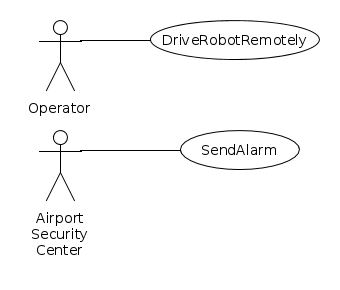
\includegraphics[scale=0.5]{./img/usecase.png}

\subsection{Scenarios}
\labelssec{Scenarios}
\begin{tabular}{| l | l |}
	\hline
	\textbf{Title} & DriveRobotRemotely
	\\ \hline
	\textbf{Description}  & The operator drives the robot to the suspicious bag
	\\ \hline
	\textbf{Relationships} & 
	\\ \hline
	\textbf{Actors} & Operator
	\\ \hline
	\textbf{Preconditions} & The robot is in the RBA, waiting for commands from the operator.
	\\ \hline
	\textbf{Postconditions} & The robot starts the detection phase.
	\\ \hline
	\textbf{Main scenario} & The operator uses the remote console to drive the robot. \\ &
	When the robot perceives the bag, it starts the detection phase.
	\\ \hline
\end{tabular}
\\
\begin{tabular}{| l | l |}
	\hline
	\textbf{Title} & SendAlarm
	\\ \hline
	\textbf{Description}  & The Airport Security Center sends an alarm signal to the robot if needed
	\\ \hline
	\textbf{Relationships} & 
	\\ \hline
	\textbf{Actors} & Airport Security Center
	\\ \hline
	\textbf{Preconditions} & The Airport Security Center received the detection results
	\\ \hline
	\textbf{Postconditions} & The robot blinks its led until it comes back to the RBA.
	\\ \hline
	\textbf{Main scenario} & 
	The Airport Security Center uses its interface to send the alarm to the robot. \\ &
	The robot blinks its led.
	\\ \hline
\end{tabular}

%\subsection{Requirements model}
%\labelssec{Requirements model}

\subsection{Domain model}
\labelssec{Domain model}
In this phase we try to find an agreement with the client on what the entities mentioned in the requirements are.\\The system is composed by three parts:
\begin{itemize}
\item \textbf{Operator's remote console}
\item \textbf{Airport Security Center's remote console}
\item \textbf{Differential drive robot}
\end{itemize}
A \textbf{console} is a physical or virtual device that allows communication between the system and an external entity. It can get user input data and send them to the system, show some system output data to the user or both. In this case, the operator's console can get input from the operator and the Airport Security Center's console can receive the detection results and emit an alarm signal.
\\A \textbf{differential drive robot} is a composed entity that is able to use some devices to perform actions and receive data from the environment. It can also communicate with other parts of the system. All differential drive robots must have a sonar and are able to move in the environment. In this case, the differential drive robot has DC motors and wheels to move, a sonar and a led.
DC motors, wheels, led and sonar are the hardware components mounted on the robot.
\\A \textbf{DC motor} can spin the attached wheel clockwise or counter-clockwise.
\\A \textbf{led} can be turned on or off.
\\A \textbf{sonar} can send an ultrasonic signal (trigger) and generates a corresponding response waveform (echo). The waveform analysis allows to estimate the distance from an obstacle.
%\subsection{System model}

\subsection{Test plan}

%===========================================================================
\section{Problem analysis}
\labelsec{ProblemAnalysis}
%===========================================================================
\subsection{Logic architecture}
%Copia pippone sulle 3 dimensioni dal suo sito

\begin{enumerate}
\item Structure:
\begin{itemize}
\item \textbf{DriveRobot} differential drive (two motor-wheels) robot equipped with a sonar.
\item \textbf{Operator Interface} used by the operator to drive the robot to the suspicious bag.
\item \textbf{ASCConsole} allows the Airport Security Center to receive the results of the detection phase and to emit alarm signal
\end{itemize}
\item Interaction: 
\item Behaviour:
\end{enumerate}
\subsection{Abstraction gap}
\subsection{Risk analysis}

%===========================================================================
\section{Work plan}
\labelsec{wplan}
%===========================================================================

%===========================================================================
\section{Project}
\labelsec{Project}
%===========================================================================

\subsection{Structure}
\subsection{Interaction}
\subsection{Behavior}

%===========================================================================
\section{Implementation}
\labelsec{Implementation}
%===========================================================================

%===========================================================================
\section{Testing}
\labelsec{testing}
%===========================================================================

%===========================================================================
\section{Deployment}
\labelsec{Deployment}
%===========================================================================

%===========================================================================
\section{Maintenance}
\labelsec{Maintenance}
%===========================================================================
\newpage
See \cite{natMol09} until page 11 (\texttt{CMM}) and pages 96-105.

%===========================================================================
\section{Information about the author}
\labelsec{Author}
%===========================================================================

\vskip.5cm
%%% \begin{figure}
\begin{tabular}{ | c |  }
\hline
  % after \\: \hline or \cline{col1-col2} \cline{col3-col4} ...
  Paolo Sarti 
  \\
   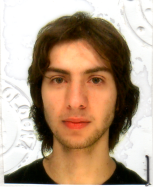
\includegraphics[scale = 0.7]{img/author_scaled.png}
  \\
\hline
\end{tabular}
\begin{tabular}{ | c |  }
\hline
  % after \\: \hline or \cline{col1-col2} \cline{col3-col4} ...
  Marcello Ballanti 
  \\

   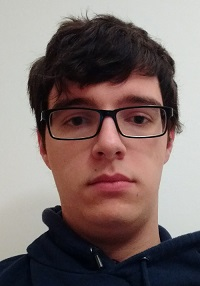
\includegraphics[scale = 0.35]{img/io2.jpg}
  \\
\hline
\end{tabular}


%%% \begin{itemize}
%%% \item Titolo di studio:\\ \\
%%% \item Interessi particolari:\\ \\
%%% \item Ha sostenuto fino ad oggi il seguente numero di esami:\\ \\
%%% \item Deve ancora sostenere i seguenti esami del I anno:\\ \\
%%% \item Prevede di svolgere un tirocinio presso:\\ \\
%%% \item Prevede di laurearsi nella sessione:\\ \\
%%% \item Intende proseguire gli studi per conseguire: \\  \\  \\
%%%   	presso la sede universitaria di: \\ \\
%%% \item Intende entrare subito nel mondo del lavoro presso : \\ \\
%%% \end{itemize}

 
\appendix


\bibliographystyle{abbrv}
\bibliography{biblio}

\end{document}












